\begin{figure*}[!t]
    \centering
    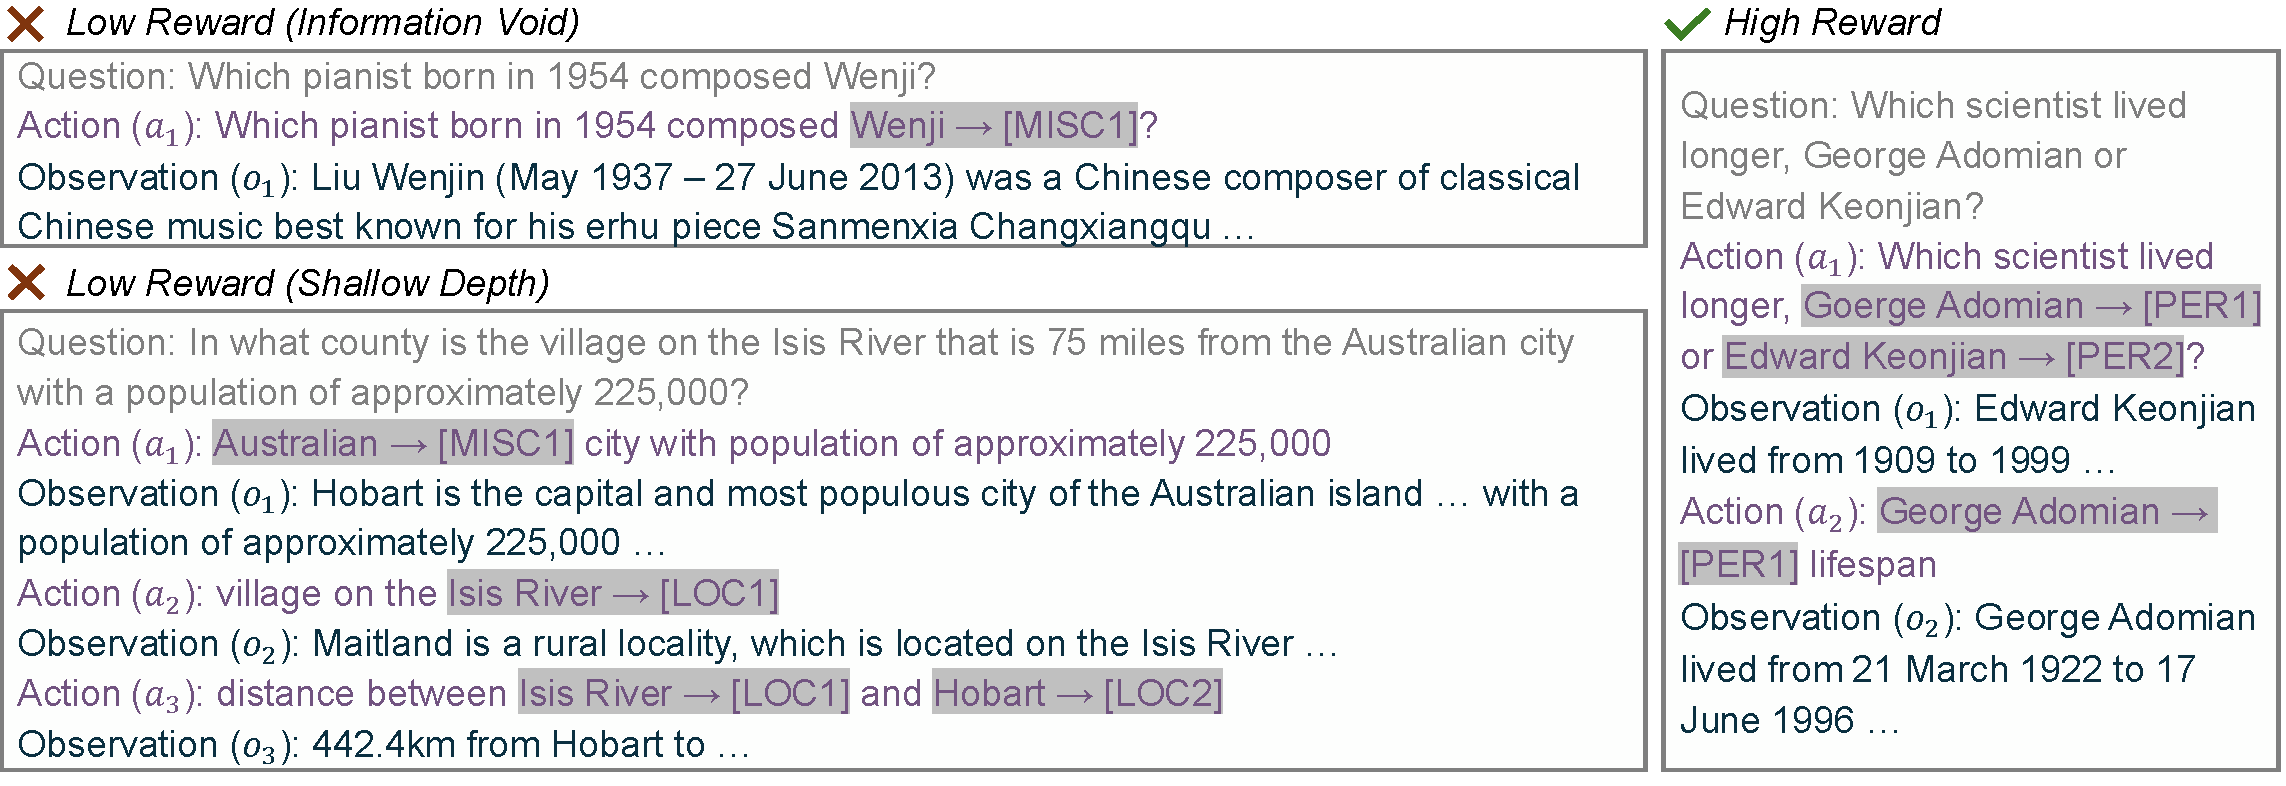
\includegraphics[width=1\linewidth]{img/ccs_qualitative_analysis.pdf}
    \caption{\textbf{Qualitative analysis of search trajectories.} CCS assigns low rewards to trajectories exhibiting (a) Information Void, where the retrieved observations fail to satisfy key entity constraints, and (b) Shallow Depth, where the agent fails to complete the full multi-hop search scaffold. By contrast, high rewards are assigned only to trajectories that preserve both the search structure and the supporting observations needed to faithfully reconstruct the original question. Masked spans are highlighted in gray.}
    \label{fig:qualitative_analysis}
\end{figure*}